% --------------------------------------- godthem256 ---------------------------------------

\subsection{Image \texttt{godthem256}}

\begin{figure}[H]
	\centering
  \scalebox{0.8}{% This file was created by matlab2tikz.
%
%The latest updates can be retrieved from
%  http://www.mathworks.com/matlabcentral/fileexchange/22022-matlab2tikz-matlab2tikz
%where you can also make suggestions and rate matlab2tikz.
%
\begin{tikzpicture}

\begin{axis}[%
width=2.402in,
height=2.402in,
at={(10.142in,7.896in)},
scale only axis,
axis on top,
separate axis lines,
every outer x axis line/.append style={black},
every x tick label/.append style={font=\color{black}},
xmin=0.5,
xmax=256.5,
every outer y axis line/.append style={black},
every y tick label/.append style={font=\color{black}},
y dir=reverse,
ymin=0.5,
ymax=256.5,
hide axis
]
\addplot [forget plot] graphics [xmin=0.5,xmax=256.5,ymin=0.5,ymax=256.5] {./images/Q5/smoothed-1.png};
\end{axis}

\begin{axis}[%
width=2.402in,
height=2.402in,
at={(14.536in,7.896in)},
scale only axis,
axis on top,
separate axis lines,
every outer x axis line/.append style={black},
every x tick label/.append style={font=\color{black}},
xmin=0.5,
xmax=256.5,
every outer y axis line/.append style={black},
every y tick label/.append style={font=\color{black}},
y dir=reverse,
ymin=0.5,
ymax=256.5,
hide axis
]
\addplot [forget plot] graphics [xmin=0.5,xmax=256.5,ymin=0.5,ymax=256.5] {./images/Q5/smoothed-2.png};
\end{axis}

\begin{axis}[%
width=2.402in,
height=2.402in,
at={(10.142in,4.561in)},
scale only axis,
axis on top,
separate axis lines,
every outer x axis line/.append style={black},
every x tick label/.append style={font=\color{black}},
xmin=0.5,
xmax=256.5,
every outer y axis line/.append style={black},
every y tick label/.append style={font=\color{black}},
y dir=reverse,
ymin=0.5,
ymax=256.5,
hide axis
]
\addplot [forget plot] graphics [xmin=0.5,xmax=256.5,ymin=0.5,ymax=256.5] {./images/Q5/smoothed-3.png};
\end{axis}

\begin{axis}[%
width=2.402in,
height=2.402in,
at={(14.536in,4.561in)},
scale only axis,
axis on top,
separate axis lines,
every outer x axis line/.append style={black},
every x tick label/.append style={font=\color{black}},
xmin=0.5,
xmax=256.5,
every outer y axis line/.append style={black},
every y tick label/.append style={font=\color{black}},
y dir=reverse,
ymin=0.5,
ymax=256.5,
hide axis
]
\addplot [forget plot] graphics [xmin=0.5,xmax=256.5,ymin=0.5,ymax=256.5] {./images/Q5/smoothed-4.png};
\end{axis}

\begin{axis}[%
width=2.402in,
height=2.402in,
at={(10.142in,1.225in)},
scale only axis,
axis on top,
separate axis lines,
every outer x axis line/.append style={black},
every x tick label/.append style={font=\color{black}},
xmin=0.5,
xmax=256.5,
every outer y axis line/.append style={black},
every y tick label/.append style={font=\color{black}},
y dir=reverse,
ymin=0.5,
ymax=256.5,
hide axis
]
\addplot [forget plot] graphics [xmin=0.5,xmax=256.5,ymin=0.5,ymax=256.5] {./images/Q5/smoothed-5.png};
\end{axis}

\begin{axis}[%
width=2.402in,
height=2.402in,
at={(14.536in,1.225in)},
scale only axis,
axis on top,
separate axis lines,
every outer x axis line/.append style={black},
every x tick label/.append style={font=\color{black}},
xmin=0.5,
xmax=256.5,
every outer y axis line/.append style={black},
every y tick label/.append style={font=\color{black}},
y dir=reverse,
ymin=0.5,
ymax=256.5,
hide axis
]
\addplot [forget plot] graphics [xmin=0.5,xmax=256.5,ymin=0.5,ymax=256.5] {./images/Q5/smoothed-6.png};
\end{axis}
\end{tikzpicture}%
}
  \caption{The origin image \texttt{godthem256} (upper left) and its smoothed variants.
    From left to right and top to bottom: \texttt{scale}=$0.0001, 1, 4, 16, 64$.}
	\label{fig:Q4_smoothed_house}
\end{figure}


\begin{figure}[H]
	\centering
	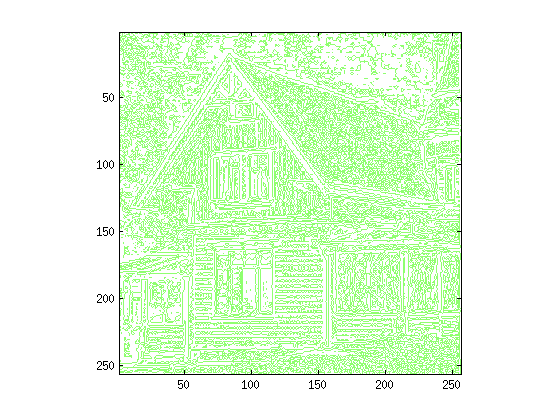
\includegraphics[scale=0.8]{./images/Q4/vv/0.0001.png}
	\caption{Zero crossings of the second derivative for image \texttt{godthem256}. $scale = 0.0001$.}
	\label{fig:Q4_vv_0.0001}
\end{figure}

\begin{figure}[H]
	\centering
	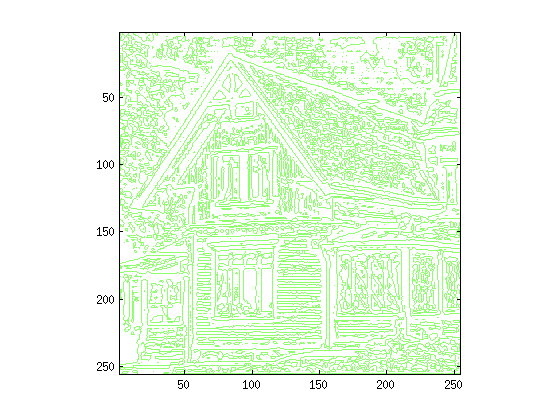
\includegraphics[scale=0.8]{./images/Q4/vv/1.png}
	\caption{Zero crossings of the second derivative for image \texttt{godthem256}. $scale = 1$.}
	\label{fig:Q4_vv_1}
\end{figure}

\begin{figure}[H]
	\centering
	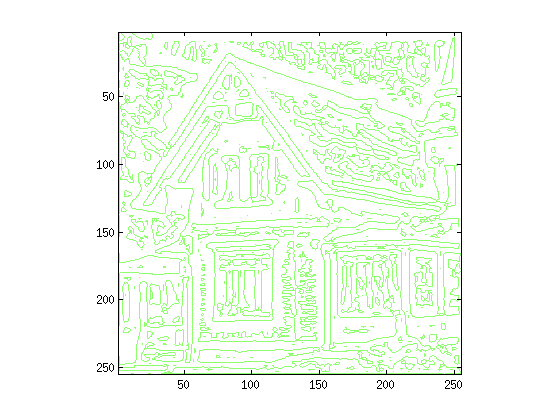
\includegraphics[scale=0.8]{./images/Q4/vv/4.png}
	\caption{Zero crossings of the second derivative for image \texttt{godthem256}. $scale = 4$.}
	\label{fig:Q4_vv_4}
\end{figure}

\begin{figure}[H]
	\centering
	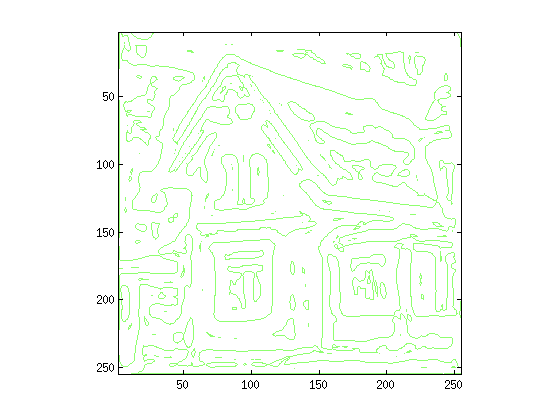
\includegraphics[scale=0.8]{./images/Q4/vv/16.png}
	\caption{Zero crossings of the second derivative for image \texttt{godthem256}. $scale = 16$.}
	\label{fig:Q4_vv_16}
\end{figure}

\begin{figure}[H]
	\centering
	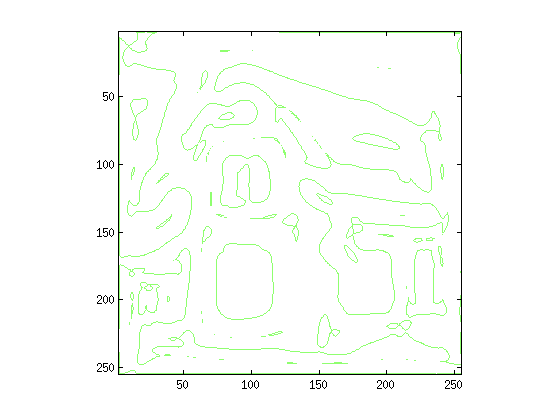
\includegraphics[scale=0.8]{./images/Q4/vv/64.png}
	\caption{Zero crossings of the second derivative for image \texttt{godthem256}. $scale = 64$.}
	\label{fig:Q4_vv_64}
\end{figure}


\begin{figure}[H]
	\centering
	\scalebox{0.8}{% This file was created by matlab2tikz.
%
%The latest updates can be retrieved from
%  http://www.mathworks.com/matlabcentral/fileexchange/22022-matlab2tikz-matlab2tikz
%where you can also make suggestions and rate matlab2tikz.
%
\begin{tikzpicture}

\begin{axis}[%
width=2.402in,
height=2.402in,
at={(8.142in,7.896in)},
scale only axis,
axis on top,
separate axis lines,
every outer x axis line/.append style={black},
every x tick label/.append style={font=\color{black}},
xmin=0.5,
xmax=256.5,
every outer y axis line/.append style={black},
every y tick label/.append style={font=\color{black}},
y dir=reverse,
ymin=0.5,
ymax=256.5,
hide axis,
title={Sign of the third order derivative. White means negative. scale = 0.0001}
]
\addplot [forget plot] graphics [xmin=0.5,xmax=256.5,ymin=0.5,ymax=256.5] {./images/Q4/vvv/house-1.png};
\end{axis}

\begin{axis}[%
width=2.402in,
height=2.402in,
at={(14.536in,7.896in)},
scale only axis,
axis on top,
separate axis lines,
every outer x axis line/.append style={black},
every x tick label/.append style={font=\color{black}},
xmin=0.5,
xmax=256.5,
every outer y axis line/.append style={black},
every y tick label/.append style={font=\color{black}},
y dir=reverse,
ymin=0.5,
ymax=256.5,
hide axis,
title={Sign of the third order derivative. White means negative. scale = 1}
]
\addplot [forget plot] graphics [xmin=0.5,xmax=256.5,ymin=0.5,ymax=256.5] {./images/Q4/vvv/house-2.png};
\end{axis}

\begin{axis}[%
width=2.402in,
height=2.402in,
at={(8.142in,4.561in)},
scale only axis,
axis on top,
separate axis lines,
every outer x axis line/.append style={black},
every x tick label/.append style={font=\color{black}},
xmin=0.5,
xmax=256.5,
every outer y axis line/.append style={black},
every y tick label/.append style={font=\color{black}},
y dir=reverse,
ymin=0.5,
ymax=256.5,
hide axis,
title={Sign of the third order derivative. White means negative. scale = 4}
]
\addplot [forget plot] graphics [xmin=0.5,xmax=256.5,ymin=0.5,ymax=256.5] {./images/Q4/vvv/house-3.png};
\end{axis}

\begin{axis}[%
width=2.402in,
height=2.402in,
at={(14.536in,4.561in)},
scale only axis,
axis on top,
separate axis lines,
every outer x axis line/.append style={black},
every x tick label/.append style={font=\color{black}},
xmin=0.5,
xmax=256.5,
every outer y axis line/.append style={black},
every y tick label/.append style={font=\color{black}},
y dir=reverse,
ymin=0.5,
ymax=256.5,
hide axis,
title={Sign of the third order derivative. White means negative. scale = 16}
]
\addplot [forget plot] graphics [xmin=0.5,xmax=256.5,ymin=0.5,ymax=256.5] {./images/Q4/vvv/house-4.png};
\end{axis}

\begin{axis}[%
width=2.402in,
height=2.402in,
at={(8.142in,1.225in)},
scale only axis,
axis on top,
separate axis lines,
every outer x axis line/.append style={black},
every x tick label/.append style={font=\color{black}},
xmin=0.5,
xmax=256.5,
every outer y axis line/.append style={black},
every y tick label/.append style={font=\color{black}},
y dir=reverse,
ymin=0.5,
ymax=256.5,
hide axis,
title={Sign of the third order derivative. White means negative. scale = 64}
]
\addplot [forget plot] graphics [xmin=0.5,xmax=256.5,ymin=0.5,ymax=256.5] {./images/Q4/vvv/house-5.png};
\end{axis}
\end{tikzpicture}%}
	\caption{Sign of the third order derivative for image \texttt{godthem256}. From upper left to lower right: $scale = 0.0001, 1, 4, 16, 64$.}
	\label{fig:Q4_vvv_}
\end{figure}


% --------------------------------------- few256 ---------------------------------------
\subsection{Image \texttt{few256}}

\begin{figure}[H]
	\centering
  \scalebox{0.8}{% This file was created by matlab2tikz.
%
%The latest updates can be retrieved from
%  http://www.mathworks.com/matlabcentral/fileexchange/22022-matlab2tikz-matlab2tikz
%where you can also make suggestions and rate matlab2tikz.
%
\begin{tikzpicture}

\begin{axis}[%
width=2.402in,
height=2.402in,
at={(10.142in,7.896in)},
scale only axis,
axis on top,
separate axis lines,
every outer x axis line/.append style={black},
every x tick label/.append style={font=\color{black}},
xmin=0.5,
xmax=256.5,
every outer y axis line/.append style={black},
every y tick label/.append style={font=\color{black}},
y dir=reverse,
ymin=0.5,
ymax=256.5,
hide axis
]
\addplot [forget plot] graphics [xmin=0.5,xmax=256.5,ymin=0.5,ymax=256.5] {./images/Q5/smoothed-1.png};
\end{axis}

\begin{axis}[%
width=2.402in,
height=2.402in,
at={(14.536in,7.896in)},
scale only axis,
axis on top,
separate axis lines,
every outer x axis line/.append style={black},
every x tick label/.append style={font=\color{black}},
xmin=0.5,
xmax=256.5,
every outer y axis line/.append style={black},
every y tick label/.append style={font=\color{black}},
y dir=reverse,
ymin=0.5,
ymax=256.5,
hide axis
]
\addplot [forget plot] graphics [xmin=0.5,xmax=256.5,ymin=0.5,ymax=256.5] {./images/Q5/smoothed-2.png};
\end{axis}

\begin{axis}[%
width=2.402in,
height=2.402in,
at={(10.142in,4.561in)},
scale only axis,
axis on top,
separate axis lines,
every outer x axis line/.append style={black},
every x tick label/.append style={font=\color{black}},
xmin=0.5,
xmax=256.5,
every outer y axis line/.append style={black},
every y tick label/.append style={font=\color{black}},
y dir=reverse,
ymin=0.5,
ymax=256.5,
hide axis
]
\addplot [forget plot] graphics [xmin=0.5,xmax=256.5,ymin=0.5,ymax=256.5] {./images/Q5/smoothed-3.png};
\end{axis}

\begin{axis}[%
width=2.402in,
height=2.402in,
at={(14.536in,4.561in)},
scale only axis,
axis on top,
separate axis lines,
every outer x axis line/.append style={black},
every x tick label/.append style={font=\color{black}},
xmin=0.5,
xmax=256.5,
every outer y axis line/.append style={black},
every y tick label/.append style={font=\color{black}},
y dir=reverse,
ymin=0.5,
ymax=256.5,
hide axis
]
\addplot [forget plot] graphics [xmin=0.5,xmax=256.5,ymin=0.5,ymax=256.5] {./images/Q5/smoothed-4.png};
\end{axis}

\begin{axis}[%
width=2.402in,
height=2.402in,
at={(10.142in,1.225in)},
scale only axis,
axis on top,
separate axis lines,
every outer x axis line/.append style={black},
every x tick label/.append style={font=\color{black}},
xmin=0.5,
xmax=256.5,
every outer y axis line/.append style={black},
every y tick label/.append style={font=\color{black}},
y dir=reverse,
ymin=0.5,
ymax=256.5,
hide axis
]
\addplot [forget plot] graphics [xmin=0.5,xmax=256.5,ymin=0.5,ymax=256.5] {./images/Q5/smoothed-5.png};
\end{axis}

\begin{axis}[%
width=2.402in,
height=2.402in,
at={(14.536in,1.225in)},
scale only axis,
axis on top,
separate axis lines,
every outer x axis line/.append style={black},
every x tick label/.append style={font=\color{black}},
xmin=0.5,
xmax=256.5,
every outer y axis line/.append style={black},
every y tick label/.append style={font=\color{black}},
y dir=reverse,
ymin=0.5,
ymax=256.5,
hide axis
]
\addplot [forget plot] graphics [xmin=0.5,xmax=256.5,ymin=0.5,ymax=256.5] {./images/Q5/smoothed-6.png};
\end{axis}
\end{tikzpicture}%
}
  \caption{The origin image \texttt{few256} (upper left) and its smoothed variants.
    From left to right and top to bottom: \texttt{scale}=$0.0001, 1, 4, 16, 64$.}
	\label{fig:Q5_smoothed_few256}
\end{figure}

\begin{figure}[H]
	\centering
	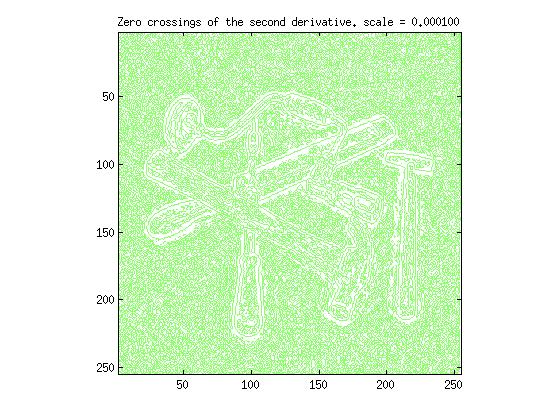
\includegraphics[scale=0.8]{./images/Q5/vv/0.0001.png}
	\caption{Zero crossings of the second derivative for image \texttt{few256}. $scale = 0.0001$.}
	\label{fig:Q5_vv_0.0001}
\end{figure}

\begin{figure}[H]
	\centering
	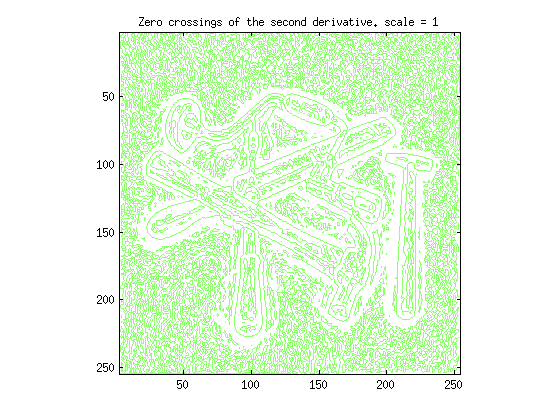
\includegraphics[scale=0.8]{./images/Q5/vv/1.png}
	\caption{Zero crossings of the second derivative for image \texttt{few256}. $scale = 1$.}
	\label{fig:Q5_vv_1}
\end{figure}

\begin{figure}[H]
	\centering
	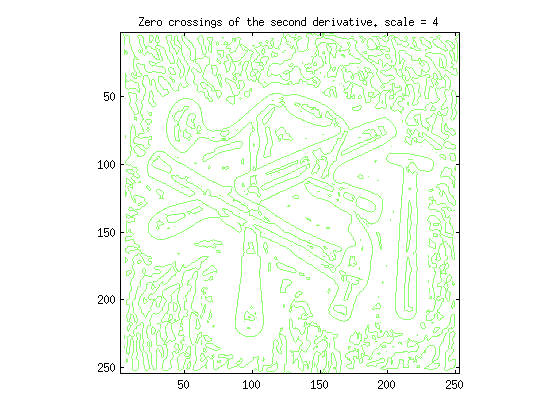
\includegraphics[scale=0.8]{./images/Q5/vv/4.png}
	\caption{Zero crossings of the second derivative for image \texttt{few256}. $scale = 4$.}
	\label{fig:Q5_vv_4}
\end{figure}

\begin{figure}[H]
	\centering
	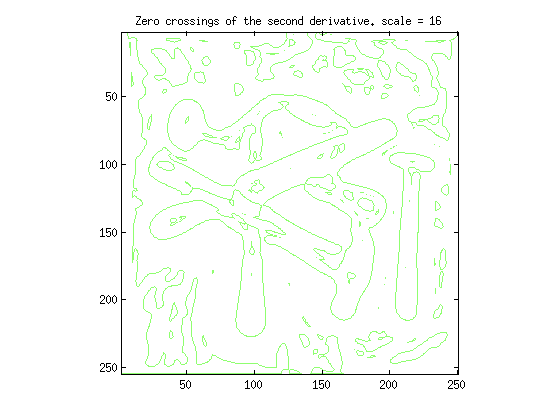
\includegraphics[scale=0.8]{./images/Q5/vv/16.png}
	\caption{Zero crossings of the second derivative for image \texttt{few256}. $scale = 16$.}
	\label{fig:Q5_vv_16}
\end{figure}

\begin{figure}[H]
	\centering
	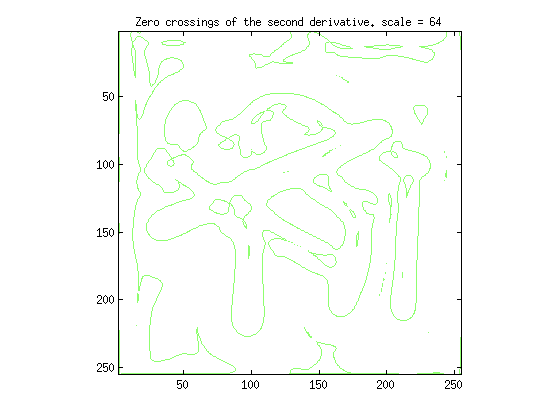
\includegraphics[scale=0.8]{./images/Q5/vv/64.png}
	\caption{Zero crossings of the second derivative for image \texttt{few256}. $scale = 64$.}
	\label{fig:Q5_vv_64}
\end{figure}


\begin{figure}[H]
	\centering
	\scalebox{0.8}{% This file was created by matlab2tikz.
%
%The latest updates can be retrieved from
%  http://www.mathworks.com/matlabcentral/fileexchange/22022-matlab2tikz-matlab2tikz
%where you can also make suggestions and rate matlab2tikz.
%
\begin{tikzpicture}

\begin{axis}[%
width=2.402in,
height=2.402in,
at={(8.142in,7.896in)},
scale only axis,
axis on top,
separate axis lines,
every outer x axis line/.append style={black},
every x tick label/.append style={font=\color{black}},
xmin=0.5,
xmax=256.5,
every outer y axis line/.append style={black},
every y tick label/.append style={font=\color{black}},
y dir=reverse,
ymin=0.5,
ymax=256.5,
hide axis,
title={Sign of the third order derivative. White means negative. scale = 0.0001}
]
\addplot [forget plot] graphics [xmin=0.5,xmax=256.5,ymin=0.5,ymax=256.5] {./images/Q5/vvv/tools-1.png};
\end{axis}

\begin{axis}[%
width=2.402in,
height=2.402in,
at={(14.536in,7.896in)},
scale only axis,
axis on top,
separate axis lines,
every outer x axis line/.append style={black},
every x tick label/.append style={font=\color{black}},
xmin=0.5,
xmax=256.5,
every outer y axis line/.append style={black},
every y tick label/.append style={font=\color{black}},
y dir=reverse,
ymin=0.5,
ymax=256.5,
hide axis,
title={Sign of the third order derivative. White means negative. scale = 1}
]
\addplot [forget plot] graphics [xmin=0.5,xmax=256.5,ymin=0.5,ymax=256.5] {./images/Q5/vvv/tools-2.png};
\end{axis}

\begin{axis}[%
width=2.402in,
height=2.402in,
at={(8.142in,4.561in)},
scale only axis,
axis on top,
separate axis lines,
every outer x axis line/.append style={black},
every x tick label/.append style={font=\color{black}},
xmin=0.5,
xmax=256.5,
every outer y axis line/.append style={black},
every y tick label/.append style={font=\color{black}},
y dir=reverse,
ymin=0.5,
ymax=256.5,
hide axis,
title={Sign of the third order derivative. White means negative. scale = 4}
]
\addplot [forget plot] graphics [xmin=0.5,xmax=256.5,ymin=0.5,ymax=256.5] {./images/Q5/vvv/tools-3.png};
\end{axis}

\begin{axis}[%
width=2.402in,
height=2.402in,
at={(14.536in,4.561in)},
scale only axis,
axis on top,
separate axis lines,
every outer x axis line/.append style={black},
every x tick label/.append style={font=\color{black}},
xmin=0.5,
xmax=256.5,
every outer y axis line/.append style={black},
every y tick label/.append style={font=\color{black}},
y dir=reverse,
ymin=0.5,
ymax=256.5,
hide axis,
title={Sign of the third order derivative. White means negative. scale = 16}
]
\addplot [forget plot] graphics [xmin=0.5,xmax=256.5,ymin=0.5,ymax=256.5] {./images/Q5/vvv/tools-4.png};
\end{axis}

\begin{axis}[%
width=2.402in,
height=2.402in,
at={(8.142in,1.225in)},
scale only axis,
axis on top,
separate axis lines,
every outer x axis line/.append style={black},
every x tick label/.append style={font=\color{black}},
xmin=0.5,
xmax=256.5,
every outer y axis line/.append style={black},
every y tick label/.append style={font=\color{black}},
y dir=reverse,
ymin=0.5,
ymax=256.5,
hide axis,
title={Sign of the third order derivative. White means negative. scale = 64}
]
\addplot [forget plot] graphics [xmin=0.5,xmax=256.5,ymin=0.5,ymax=256.5] {./images/Q5/vvv/tools-5.png};
\end{axis}
\end{tikzpicture}%}
	\caption{Sign of the third order derivative for image \texttt{few256}. From upper left to lower right: $scale = 0.0001, 1, 4, 16, 64$.}
	\label{fig:Q5_vvv_}
\end{figure}



\subsection{Question 4}

Figures \ref{fig:Q4_vv_0.0001} - \ref{fig:Q4_vv_64} and
\ref{fig:Q5_vv_0.0001} - \ref{fig:Q5_vv_64} illustrate the points where
the second order derivative of the \texttt{godthem256} and \texttt{few256} images
is zero for different values of $scale$. What is apparent here is that the higher the $scale$,
that is the higher the variance of the gaussian filter used, the more the blurring
in the image. The higher the blurring the higher suppression of the noise
present in the image (that is the reason why spurious lines diminish for
increasing values for scale), but also the lower the accuracy at approximating
the true position of the edges. If blurring is performed in a high degree,
edges of interest may disappear and thus not be located,
or located, but with a certain drop in accuracy, since what is approximated are
\textit{points} where the gradient magnitude is at maximum at the gradient's direction,
and the shape of the edge is distorted due to the blurring.


\subsection{Question 5}

Figures \ref{fig:Q4_vvv_} and \ref{fig:Q5_vvv_} illustrate the points where the
third order derivative of the \texttt{godthem256} and \texttt{few256} images
is negative for different values of $scale$. What is apparent here is that
the higher the blurring degree, the coarser, or, thicker the various edges
become.

\subsection{Question 6}

As stated in the assignment notes, the gradient magnitude reaches a local
maximum where the second order derivative $L_{vv} = 0$ \textit{and} $L_{vvv} < 0$.
Hence we can combine these two pieces of information in order to improve on the
response of plain $L_{vv}$. Figures \ref{fig:Q6_tools} and \ref{fig:Q6_house}
illustrate the results of an operation using the aforementioned pieces of
information for images \texttt{few256} and \texttt{godthem256} for a
$scale$ factor of $4$.


\begin{figure}[H]
	\centering
	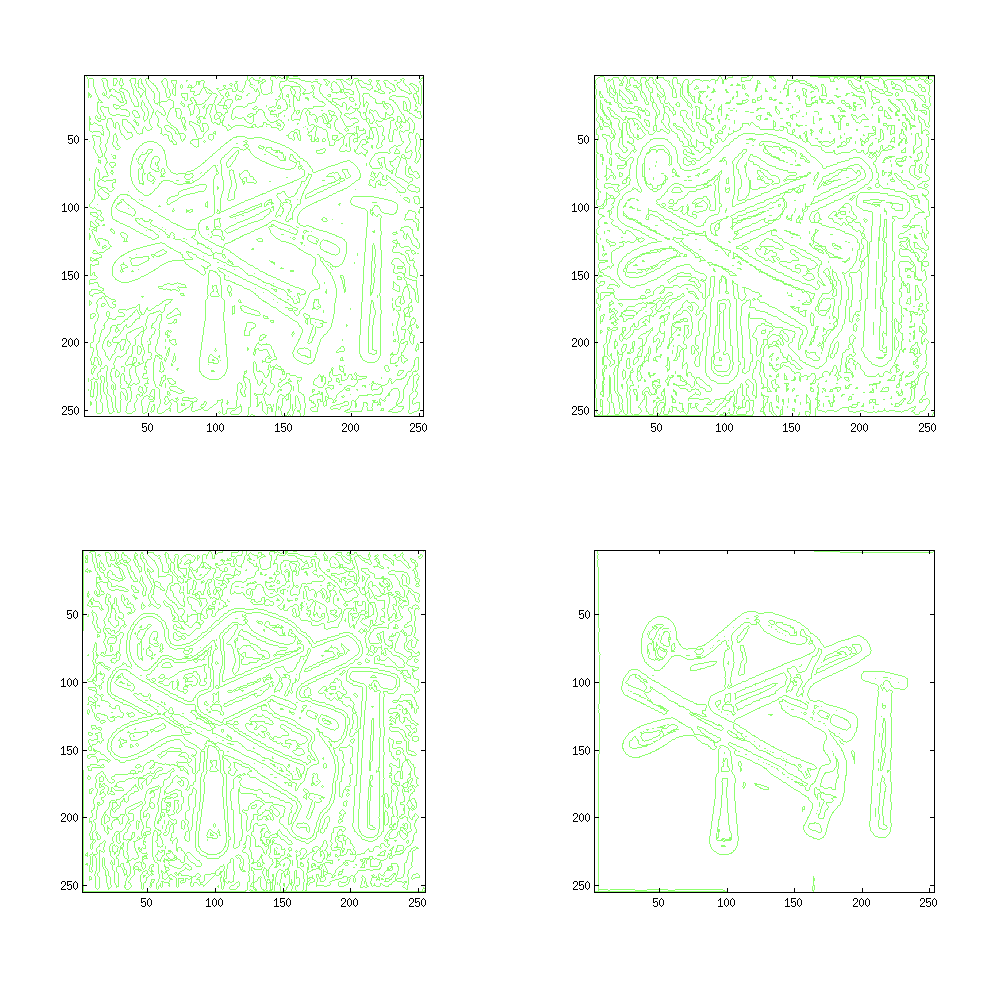
\includegraphics[scale=0.6]{./images/Q6/tools_combo.png}
  \caption{The result of combining both $Lvv = 0$ and $Lvvv < 0$ on image \texttt{few256}.}
	\label{fig:Q6_tools}
\end{figure}

\begin{figure}[H]
	\centering
	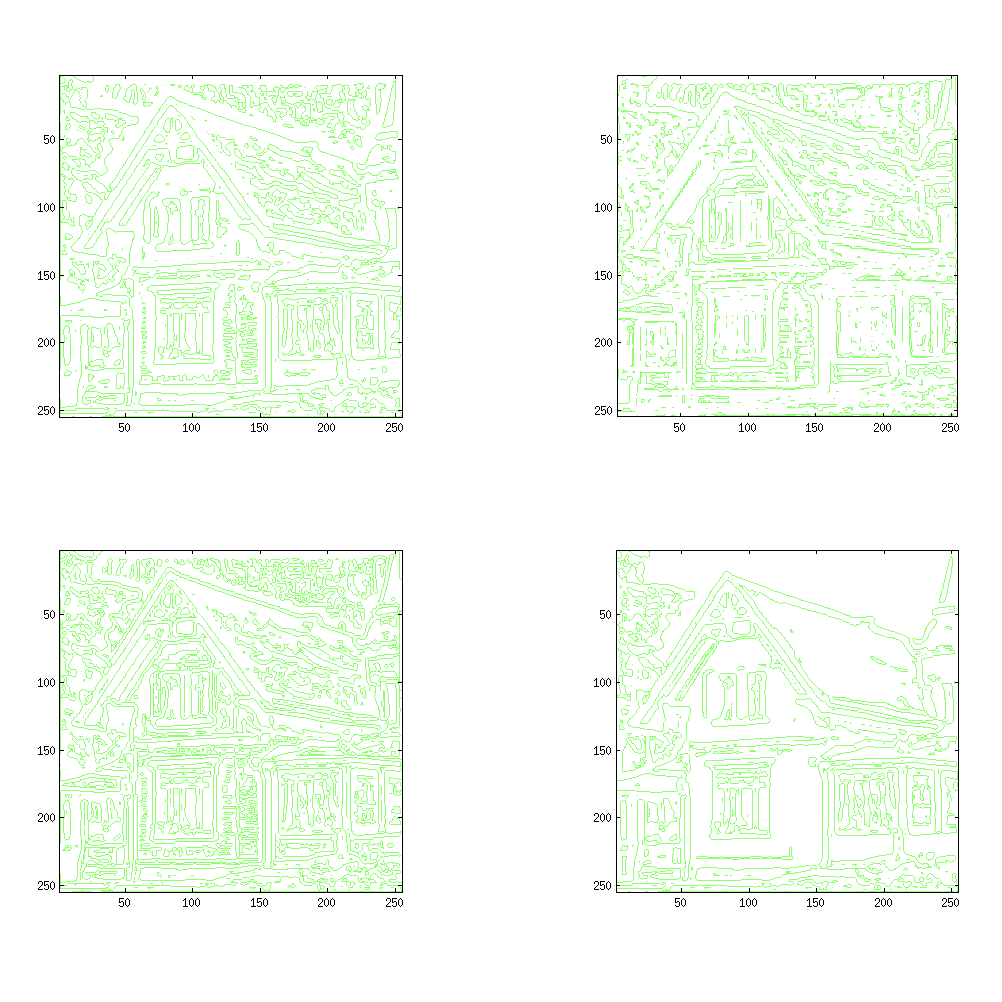
\includegraphics[scale=0.6]{./images/Q6/house_combo.png}
  \caption{The result of combining both $Lvv = 0$ and $Lvvv < 0$ on image \texttt{godthem256}.}
	\label{fig:Q6_house}
\end{figure}


